\documentclass[12pt]{article}
\usepackage{sbc-template}
\usepackage{graphicx,url}
%\usepackage[brazil]{babel}   
\usepackage[utf8]{inputenc}    
\usepackage{amsmath}
\usepackage[brazil]{babel} 
\usepackage{placeins}     
\usepackage{hyperref}
\usepackage[usenames, dvipsnames]{color}
\usepackage{listings}
\lstdefinestyle{sharpc}{language=[Sharp]C, frame=lr, rulecolor=\color{blue!80!black}}
\sloppy

\title{Estudo de Caso: Aplicação de Sistemas ETL como fonte provedora de dados do transporte coletivo na cidade de Manaus.}
\author{}
\address{}


\begin{document} 

\maketitle
\textit{}
\hspace*{\fill} Edilson Galvão dos santos Júnior\\
\hspace*{\fill} MBA em Projeto de Aplicações .NET\\
\hspace*{\fill} Professor orientador: Dr. Aniceto C. De Andrade Júnior\\

\noindent \textbf{Resumo}\\
Lorem ipsum dolor sit amet, consectetur adipiscing elit, sed do eiusmod tempor incididunt ut labore et dolore magna aliqua. Ut enim ad minim veniam, quis nostrud exercitation ullamco laboris nisi ut aliquip ex ea commodo consequat. Duis aute irure dolor in reprehenderit in voluptate velit esse cillum dolore eu fugiat nulla pariatur. Excepteur sint occaecat cupidatat non proident, sunt in culpa qui officia deserunt mollit anim id est laborum.\\
\textbf{Palavras-chave:} Inicie aqui as palavras-chave, sempre com a letra inicial em maiúscula - Fonte Arial tamanho 12 - Use Espaço simples entre linhas – Alinhamento justificado.

\noindent \textbf{Abstract}\\
Lorem ipsum dolor sit amet, consectetur adipiscing elit, sed do eiusmod tempor incididunt ut labore et dolore magna aliqua. Ut enim ad minim veniam, quis nostrud exercitation ullamco laboris nisi ut aliquip ex ea commodo consequat. Duis aute irure dolor in reprehenderit in voluptate velit esse cillum dolore eu fugiat nulla pariatur. Excepteur sint occaecat cupidatat non proident, sunt in culpa qui officia deserunt mollit anim id est laborum.\\
\textbf{Keywords:} Tradução das palavras-chave para a mesma língua do Abstract. Mesmas considerações de formatação para as Palavras-chave.

\section{Introdução}

\section{Metodologia} \label{sec:firstpage}
Esta seção descreve a metodologia aplicada neste artigo, para tal, quatro ciclos de trabalho foram executados: O primeiro ciclo envolve o estudo das tecnologias atuais e de suas respectivas bibliografias, em um segundo momento, a partir do estudo foi escolhido um conjunto de ferramenta, entre elas podemos citar: Banco de dados, tecnologias com suporte a multiplataforma, servidores de hospedagem entre outros, portanto, o terceiro ciclo baseou-se nessas tecnologias para criar um modelo de dados e propor soluções para o transporte coletivo no que tange a disponibilização de informação, e por fim, fez-se uma analise sob os dados coletados. Cada fase é descrita sequencialmente em uma ordem cronológica. 

\begin{enumerate}
\item A primeira fase consistiu em uma busca exploratória para reconhecer bibliografias, aplicativos e tecnologias compatíveis com o cenário proposto neste trabalho. Os estudos carregam com si análises sobre as tecnologia que podem ser aplicadas e o impacto de cada uma. A ideia principal por trás dessa fase é reconhecer um padrão, e analisar como este é aplicado como produto final ou como camada intermediária para outros fins.\\

\item A Segunda fase foi a definição das tecnologias de captura de dados através da internet, a transmissão dos dados entre os servidores e serviços, o tratamento e enriquecimento dos dados, o armazenamento do conteúdo processado e, por fim, a exposição do conteúdo através da internet.\\

\item A Terceira fase foi o desenvolvimento de uma arquitetura capaz de suportar todos os processos descritos na fase dois, alguns pontos como flexibilidade e manutenção foram fundamentais para nortear as escolhas.\\

\item A Quarta fase teve como papel analisar os dados de forma descritiva e explicativa baseando-se no modelo aqui apresentado e a sua relação com o objeto real de forma qualitativa e quantitativa. Nesta etapa é possível identificar, mensurar e demonstrar as relações entre as grandezas estudadas e como isso afeta os usuários finais do modelo.\\
\end{enumerate}

A finalidade desta pesquisa é criar um modelo de dados que possa ser exposto e consumido por diferentes tipos de aplicações, verificar a precisão das informações do modelo e realizar um contraste com a realidade da região metropolitana de manaus no que tange as informações do transporte coletivo. Uma segunda vertente desta pesquisa é expor os dados estudados e os artefatos gerados para analise de terceiros.

\section{Revisão de Literatura}
Esta seção tem como objetivo introduzir os conceitos necessários para uma melhor compreensão dos dados subsequentes e do contexto geral deste artigo. 

\subsection{Cidades Inteligentes}
São aquelas que combinam as facilidades das TICs e da Web 2.0 com os esforços organizacionais, de design e planejamento, para desmaterializar e acelerar os processos burocráticos, ajudando a identificar e implementar soluções inovadoras para o gerenciamento da complexidade das cidades. Esta definição é apresentado em uma tabela comparativa entre de definições apontada em  ~\cite{art12}.

As migrações e os fluxos de pessoas para as cidades geram grande impacto as estruturas de estado, juntamente com esses fluxos a necessidade de atendimento sob as demandas essenciais como transporte público, educação e saúde crescem ~\cite{art13}. Como cada cidade tem suas próprias demandas e estruturas, inúmeras podem ser as soluções baseadas em Tecnologia da Informação e comunicação, portanto para uma cidade inteligente existir é necessário que se tenha um conjunto tecnológico e a possibilidade de obter dados sensíveis a vida cotidiana~\cite{art12}.

Pode-se exemplificar tais ações convergente a cidades inteligentes analisando os trabalhos de ~\cite{art01} e ~\cite{art02} que criam uma infraestrutura de sistemas e se usam da exposição do dados de mobilidade urbana pelo governo para expor ao público em geral as informações do transportes coletivos. Entretanto, a implementação de TICs não pode ser considerada como única solução para resolver os problemas sociais que as cidade enfrentam.

\subsection{Data warehouse e o Processo ETL}\label{sec:ETLRev}
A ideia principal quando tratamos de data warehouse (DW) é construir uma base de dados proveniente de inúmeras outras fontes não homogêneas~\cite{art08}. São dados provisionados por diferentes fontes, onde espera-se um processamento sobre um conjunto de dados fornecidos a fim de que seja criada uma fonte uniforme. O processo de recuperar e processar as informações de diferentes lugares e condensar a estrutura de dados capturada em um DW é chamada de ETL. 

ETL (Extract, Transform and Load) é um conceito baseado em extração, transformação e carga de dados.  Segundo \cite{art04} a etapa de extração deve ser focada em extrair os conteúdos mais sensíveis para a aplicação a ser desenvolvida. Nessa fase todos os dados são recuperados de suas fontes provedoras e armazenados no DW, estes dados normalmente estão em conflito ou destoantes da realidade porque inúmeros outros processos foram executados sob si ou sob parte de suas informações ~\cite{art09}.

A transformação é um passo subsequente, neste momento realiza-se a limpeza, a filtragem e a transformação com intuito de padronizar ou melhorar os dados, observando-se sempre as regras de negócio. Nessa fase devemos garantir que as grandezas métricas como escala e as propriedades do modelo estejam em conformidade. São pilares fundamentais fatores como remoção de entradas duplicadas, ajustes na precisão dos dados e ajustes nos domínios dados.

O processo de carga, é em resumo, uma estruturação física dos dados, a forma de se armazenar e entregar dados aos meios solicitantes. Todos os processos anteriores tiveram como finalidade convergir para um modelo único que possa ser disponibilizado para camada de apresentação. É importante salientar que a carga deve ser tolerante a falha, caso ocorra falhas, não deve ser necessário reprocessar todas ou parte das fontes de dados.

\subsection{Sistemas de Propósito Similar}
No trabalho proposto por ~\cite{art01} foi desenvolvido um processo baseado em workflows ETL que processam e enriquecem os dados provido do estado do Rio de Janeiro. Foi apresentada a arquitetura, as regras ETL que foram usadas, as tecnologias de armazenamento e os entraves frente a exposição dos dados. O mesmo contexto de pesquisa foi utilizado em ~\cite{art02}.

No que tange a contexto de sistemas de informação a usuários, podemos destacar o trabalho realizado por ~\cite{art03}, as diferenças explícitas entre este e os trabalhos anteriormente citados estão na otimização da busca de linhas, a busca por informações de rotas entre pontos distintos e a cidade de Campina Grande que foi objeto do estudo.

Quando nos referimos a cidade de Manaus, os estudos em sua grande maioria são qualitativos, mensurando os sentimentos do usuário frente a mobilidade urbana como um todo. Os artigos apresentado por ~\cite{art11} e ~\cite{art10} refletem uma realidade de 12 anos atrás, mas as questões e métodos ainda são bem atuais.

\subsection{API e Serviços WEB} \label{sec:APIWEB}
API, ou \textit{Application Programming Interface} é uma interface de sistema capaz de comunicar dois aplicativos de computador usando um sistema de linguagem comum~\cite{site05}. Uma API Fornece uma interface de ligação em alto nível para utilitários ou serviços que podem ser disponibilizada via aplicativo ou internet.

Serviços WEB são um conjunto de API's baseadas em protocolos da WEB que se comunicam por meio de redes de computadores baseando-se em URI (Uniform Resource Identifier)~\cite{site06} e são definidos como blocos modulares, de estrutura independente que fornecem uma unidade lógica ou funcionalidade de negócios para aplicações por meio da internet \cite{art06}. Para trocar dados utiliza-se XML, Json ou outro formato independente de linguagem computacional~\cite{site07}.

Para resolver problemas de geoposicionamento ou capturar informação a partir de coordenada pode-se usar algumas API's disponibilizadas publicamente via internet. A \textit{API Distance Matrix} é um serviço que fornece distância e tempo de viagem para uma matriz de origens e destinos, com base na rota recomendada entre os pontos inicial e final \cite{site02}. Com as mesmas caracteristicas da API anterior, \textit{A Geocoding API} é um serviço que fornece geocodificação e geocodificação reversa de endereços\cite{site03}. 

\subsection{Banco de dados com Microsoft SQL Server}\label{sec:DBORM}
O Microsoft SQL Server é um sistema gerenciador de Banco de dados relacional (SGBD), segundo a~\cite{site04} este SGDB é o líder do setor em ODBMS (sistemas de gerenciamento de bancos de dados operacionais). Para armazenar dados usou-se como framework de suporte intermediário uma aplicação ORM denominada de Entity Framework.

O Entity Framework(EF) fornece um mecanismo flexível para mapear modelos de aplicativos de nível superior para esquemas relacionais existentes. O framework disponibiliza entre suas várias ferramentas a possibilidade de criar esquemas baseado em objeto-relacional. 

Para criar uma ligação entre os dados convertidos e o banco de dados, o EF dispõem do CodeFirst. CodeFirst é uma técnica para controlar o mapeamento de objetos e tabelas no banco de dados a partir das classes escritas no código fonte. O gerenciamento de chaves primárias e estrangeiras são feitas automaticamente, e o contexto é responsável pelas alterações do modelo.

%%%%%%%%%%%%%%%%%% ---------- Apresentação da Pesquisa --------- %%%%%%%%%%%%%%%%%%
\section{Apresentação da Pesquisa}\label{sec:horaDoShow}
Será proposto um modelo de software que explora os princípios de data Warehouse para gerar e expor dados relacionados com a mobilidade urbana. Todos os processos e tecnologias são exposto e discutidos assim como os resultados alcançados.

Para reduzir o espaço amostral e aferir de maneira mais precisa os resultados deste estudo, foi necessário focar na cidade de manaus e nas informações providas publicamente por esta no que tange a mobilidade urbana. Este trabalho explora de forma  específica um modal de transporte, o ônibus como meio coletivo.

Por meio deste visa-se propor um modelo de dados como padrão de atividade meio para fins informativos em diversas plataformas como, dispositivos móveis, sites e computadores de mesa (Windows/Linux). As tecnologias adotadas são baseadas na plataforma .NET, e contemplam .NET core 2.0, Microsoft SQL Server 2017 e Entity Framework 6.2. Serviços de geolocalização que convertem coordenadas em nomes e nomes em coordenadas são usadas para imprimir maior confiança ao modelo, além de garantir uma estimativa de tempo de chegada ao destino mais precisa.

%%%%%%%%%%%%%%%%%% ---------------- Arquitetura ---------------- %%%%%%%%%%%%%%%%%%
\subsection{Arquitetura}\label{sec:Arquitetura}
As subseções do tópico ~\ref{sec:horaDoShow} descrevem as tecnologias, arquitetura e regras utilizadas neste modelo proposto. A Figura ~\ref{fig:Arquiteura}, Condensa e traduz as subseções apresentadas em um diagrama de blocos direcionado.

\begin{figure}[ht]
\centering
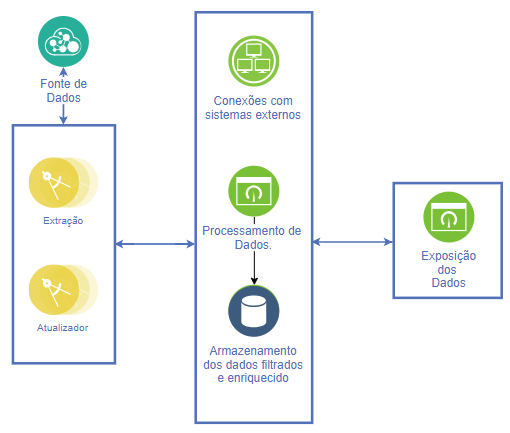
\includegraphics[width=.75\textwidth]{./Resources/arquitetura.PNG}
\caption{Abstração em bloco do modelo proposto criado pelo autor.}
\label{fig:Arquiteura}
\end{figure}

%%%%%%%%%%%%%%%%% ---------------- Fonte de Dados ---------------- %%%%%%%%%%%%%%%%%%
\subsection{Fonte de Dados}\label{sec:fontdedados}
As fontes provedoras de dados são auto suficientes quanto a publicação de dados, isso implica que o formato do arquivo e seu conteúdo são criados sem um modelo padrão. O INDA, site de Infraestrutura Nacional de Dados Abertos, que tem por objetivo a disseminação e compartilhamento de dados e informações públicas, dispõem de dados com mais de 50 tipos de extensões diferentes\cite{site01}. Portanto, dado um conjunto similar de dados é possível que se tenha N diferentes formas de arquiteturar esse conteúdo, para reduzir ou melhorar a forma como se processa essa gama de diferentes informações utilizou-se a técnica descrita na seção ~\ref{sec:ETLRev}.
     
O ícone \textit{fonte de dados} descrito na figura ~\ref{fig:Arquiteura} representa todas as formas de exposição de informações do transporte coletivo. Para o modelo específico descrito neste artigo, utilizou-se o formato JSON por ser o padrão exposto pela operadora dos dados. Entretanto, é possível recuperar diferente formatos de arquivos, como *.xml, *.gson,*.json, *.dat, *.raw, entre muitos outros, isso irá depender estritamente da fonte de dados em que se recupera os dados.

%%%%%%%%%%%%%%%%% ---------------- Extratores e Atualizadores ---------------- %%%%%%%%%%%%%%%%%%
\subsection{Extratores e Atualizadores}
No retângulo localizado a esquerda na figura~\ref{fig:Arquiteura}, tem-se as funções iniciais do Sistema que são: \textit{Extração} e \textit{Atualizador}. A função de extração é responsável por coletar todas as informações provenientes das linhas e do sistema como um todo através da \textit{fonte de dados} exposta e descrita na seção anterior. Todos os dados coletados nesta fase são armazenados temporariamente em cache e posteriormente deletado, quando a fase de refinamento estiver concluída. Todos os dados para processamento são recuperados por meio de serviços web. Na figura ~\ref{fig:Arquiteura} os pontos de coletas são: \textit{Fontes de dados} e \textit{Conexões com sistemas externos}. 

A função de atualização é responsável por verificar se alguma linha precisa ser atualizada, ou se algum dado não está mais coeso. O atualizador é responsável por capturar todo o conjunto de dados e compreender quais destes precisam de revisão. As regras adotadas no sistema presente é que os valores devem ser requisitados em um intervalo de 60 segundos, onde, caso os veículos, linhas ou outras informações estejam destoantes das armazenadas em cache, o sistema irá enviar para a central de processamento as informações capturadas e espera-se que os dados sejam atualizados.

Neste modelo o Atualizador foi implementado em um contexto distinto do qual armazena o sistema central, essa política reduz o impacto na atualização e separa em camada fisica os módulos do Atualizador, pode-se adotar esta medida como boa prática, porém não existem restrições em hospedar ambas ferramentas em um mesmo contexto ou container.

%%%%%%%%%%%%%%%%% ---------------- Conexões ---------------- %%%%%%%%%%%%%%%%%%
\subsection{Conexões Com sistemas Externos}\label{sec:sistemasexternos}
A Conexão com Sistemas Externos são estruturas que compõem o kernel do modelo e tem por finalidade enriquecer os dados provenientes da extração com recursos advindo dos meios externo a \textit{fonte de dados}. Cita-se como exemplo, dados de geoposicionamento, informações de tempo e distância referente a coordenadas ou conjunto de coordenadas, tarifas, e pontos de auxílio como estações e lojas de bilhetes.

\subsubsection{Enriquecimento através de APIs}\label{sec:api}
No que concerne a dados relativos a geolocalização este modelo se alimenta dos dados provenientes da fonte de dados descrita em ~\ref{sec:fontdedados}. Esses dados contemplam coordenadas baseadas em latitude e longitude, não são expostos dados como nome de rua e avenida, distância entre pontos e tempo médio de tráfego. Portanto, para enriquecer os dados utiliza-se APIs de terceiros como \textit{Distance Matrix} e \textit{Geocoding API} disponibilizada pelo Google. 

\textbf{Distance Matrix}: Abaixo segue o trecho em JSON dos dados recuperados pela API de um ponto A até o ponto B. Esse conteúdo é filtrado e ajustado ao modelo original assim como descrito em ~\ref{sec:REFINA}.

\lstset{					% general command to set parameter(s)
basicstyle=\small,          % print whole listing small
keywordstyle=\color{black}\bfseries\underbar,
identifierstyle=,           % nothing happens
commentstyle=\color{white}, % white comments
stringstyle=\ttfamily,
showstringspaces = false,
basicstyle=\small\ttfamily,
keywordstyle=\bfseries}
\begin{lstlisting}
{
   "destination_addresses" : [ "New York, NY, USA" ],
   "origin_addresses" : [ "Washington, DC, USA" ],
   "rows" : [ {"elements" : [{
   "distance" : { "text" : "225 mi", "value" : 361715},
   "duration" : { "text" : "3 hours 49 mins", "value" : 13725},
   "status" : "OK" }]}],
   "status" : "OK"
}
\end{lstlisting}

\textbf{Geocoding API}: Essa API se torna fundamental para o modelo, uma vez que todas as informações são baseadas em coordenadas, no trecho do JSON abaixo tem-se uma parte das informações que são usadas para o enriquecimento do modelo.

\lstset{basicstyle=\small, keywordstyle=\color{black}\bfseries\underbar,identifierstyle=,          
commentstyle=\color{white}, stringstyle=\ttfamily, showstringspaces = false,
basicstyle=\small\ttfamily, keywordstyle=\bfseries}
\begin{lstlisting}
{
  "results": [{
      "address_components": [
        {"long_name": "752", ...},
        {"long_name": "Avenida Carvalho Leal","shor...},
        {"long_name": "Cachoeirinha",...},
        {"long_name": "Manaus","short_name":...},...}]]
}
\end{lstlisting}

%%%%%%%%%%%%%%%%% ---------- Processamento, Armazenamento e Refinamento ---------- %%%%%%%%%%%%%%%%%%
\subsection{Processamento, Armazenamento e Refinamento}
O Processamento de Dados recebe os dados que foram disponibilizados pelo micro-serviço de extração, sua função é convergir o processo de ETL descrito na secção ~\ref{sec:ETLRev} com os serviços de enriquecimento descrito no tópico 'Conexão com Sistemas Externos'. Este módulo é considerado como parte principal da aplicação por orquestrar e conter a maior parte da lógica de negócio, além de sua camada conversar diretamente com todas as outras. 

Abaixo são descritos os processos que são executados durante o processamento do modelo:

\begin{enumerate}
\item Antes de qualquer requisição aos extratores, o sistema consulta sua base de dados para garantir que os dados estão desatualizados e precisam ser processados e atualizados. Uma vez que os dados estão atualizados o sistema retorna o objeto como resposta para o requisitante.\\

\item Os extratores fornecem um conjunto de instruções, as quais cita-se o nome da linha, o número da linha e uma referencia para os veículos que operam naquela rota e são definidas no JSON abaixo:

\lstset{basicstyle=\small, keywordstyle=\color{black}\bfseries\underbar,identifierstyle=,          
commentstyle=\color{white}, stringstyle=\ttfamily, showstringspaces = false,
basicstyle=\small\ttfamily, keywordstyle=\bfseries}
\begin{lstlisting}
      {"idLinha":234,"codigo":"000","nome":"Nome Linha"}
\end{lstlisting}
A referencia do arquivo acima descrito nos leva a um conjunto de automoveis, cada automovel é representado por um nome e uma coordenada baseada em latitude e longitude. A mesma referencia da linha engloba os dados de geolocalização  das estações.
\lstset{basicstyle=\small, keywordstyle=\color{black}\bfseries\underbar,identifierstyle=,          
commentstyle=\color{white}, stringstyle=\ttfamily, showstringspaces = false,
basicstyle=\small\ttfamily, keywordstyle=\bfseries}
\begin{lstlisting}
     {"veiculo":"ABCD","lat":-3.126152,"lon":-60.014391}
\end{lstlisting}

\item Os dados sobre as linhas e estações são constantes, portanto, caso a linha já exista no banco de dados, apenas as informações referentes ao automóveis serão enriquecidas. No tópico ~\ref{sec:api} são descritos as fontes e os modelos de enriquecimento da tabela \textit{Line} e de suas sub-tabelas.\\

\item os procedimento de refinamento dos dados, Armazenamento das informações no banco de dados e a exposição são descritas nas seções ~\ref{sec:REFINA},  ~\ref{sec:ADONET}, ~\ref{sec:WCFExpo} respectivamente.
\end{enumerate}

%%%%%%%%%%%%%%%%% ---------------- Refinamento e Enriquecimento---------------- %%%%%%%%%%%%%%%%%%
\subsubsection{Refinamento} \label{sec:REFINA}
O modelo proposto na figura \ref{fig:FiguraEsquemaDatabase} é o modelo ideal para demonstrar o transporte público da capital do amazonas. É fundamental refinar e enriquecer os dados provenientes das diversas fontes de dados.

A primeira técnica utilizada para remover dados não significativo ao modelo, é o POCO,
os dados são recuperados no formato JSON e são processados e convertidos para classes .NET através de Plain OLD CLR Object. A função deste tipo de classe é converter o domínio de um arquivo JSON para uma representação orientada a objeto. As entidades que não acrescentam informações são removidas da classe destino, logo, evita-se a conversão de propriedades em tempo de execução e mantém-se a classe destino coesa.  

Em um segundo momento, os dados recuperados e demonstradas em ~\ref{sec:api} são utilizados para enriquecer o modelo proposto utilizando-se da técnica demonstrada no parágrafo anterior. Toma-se de exemplo a tabela StreetName, que visa reduzir o número de consultas aos serviços externos pois armazenam conteúdo referente às coordenadas, portanto, aceleram o processo de enriquecimento e reduzem a carga de processamento do modelo. As estações e os automóveis se valem do mesmo fluxo de conversão, neste caso utiliza-se latitude e longitude como coordenadas reversas, com o intuito de recuperar dados na forma de endereço, denominações de ruas, avenidas e CEP.

%%%%%%%%%%%%%%%%% ---------------- Exposição dos Dados ---------------- %%%%%%%%%%%%%%%%%%
\subsubsection{Exposição dos Dados} \label{sec:WCFExpo}
Para expor os dados refinados utilizou-se da tecnologia WCF, Window communication Foundation, de forma nativa para apoio às ferramentas baseadas em .NET. Ao usar de forma nativa não é necessário usar técnicas de conversão de dados para classe orientadas a objeto, visto que, o próprio WCF Cria um proxy que traduz as informações WSDL em classes, isto facilita e acelera o desenvolvimento do modelo.

Sobre essa perspectiva o WCF foi desenvolvido com o intuito de funcionar bem para qualquer tipo de troca de mensagens baseadas na plataforma .NET, seu desempenho é melhor ou similar a qualquer outra opção de serviço WEB.\cite{art07}.

Foram exposto os dado seguindo o contrato descrito abaixo:
\lstset{basicstyle=\small, keywordstyle=\color{black}\bfseries\underbar,identifierstyle=,          
commentstyle=\color{white}, stringstyle=\ttfamily, showstringspaces = false,
basicstyle=\small\ttfamily, keywordstyle=\bfseries}
\begin{lstlisting}
1. List<VehicleInfo> GetAvailableLines();
2. List<Line> GetOutDated(int timeout);
3. Line UpdateLine(int lineNumber);
4. Line UpdateLine(long lat, long lon, int lineNumber);
5. StreetName GetStreeName(double lat, double lon);
6. List<RechargeCards> GetStores();
\end{lstlisting}

São expostos de forma sequencial, A lista de linhas disponíveis para consulta que são enumeradas de 0 até 999 tendo em vista a ordem do sistema de transporte descrito neste trabalho. A lista de linhas que excedem o tempo de atualizado definida em segundos. O retorno de uma linha de ônibus atualizada sem o calculo de distancia e tempo até um ponto qualquer. O retorno de uma linha de ônibus com estimativa de tempo e distancia, O nome de ruas e avenidas baseadas em uma coordenada e por fim a lista de lojas de bilhetes de transporte público.
%%%%%%%%%%%%%%%%% ---------------- ADO.NET Entity Framework ---------------- %%%%%%%%%%%%%%%%%%
\subsubsection{Armazenamento de dados} \label{sec:ADONET}
Para armazenar os dados que passaram por processo de filtragem e enriquecimento, utiliza-se o SGBD Microsoft SQL Server. A versão MS-SQL 2017 foi escolhidapor ter suporte a instalação em servidores linux e dar suporte a infraestrutura de aplicativos .NET.

O Modelo descrito nesse artigo utiliza o Entity Framework como ORM para criação, manipulação e manutenção dos dados e tabelas. Portanto, todas as interações entre os dados e a aplicação são gerenciados por classes especificas do sistema, isso reduz a complexidade da criação do banco de dados e da manutenção de suas tabelas.

\begin{figure}[h!]
\centering
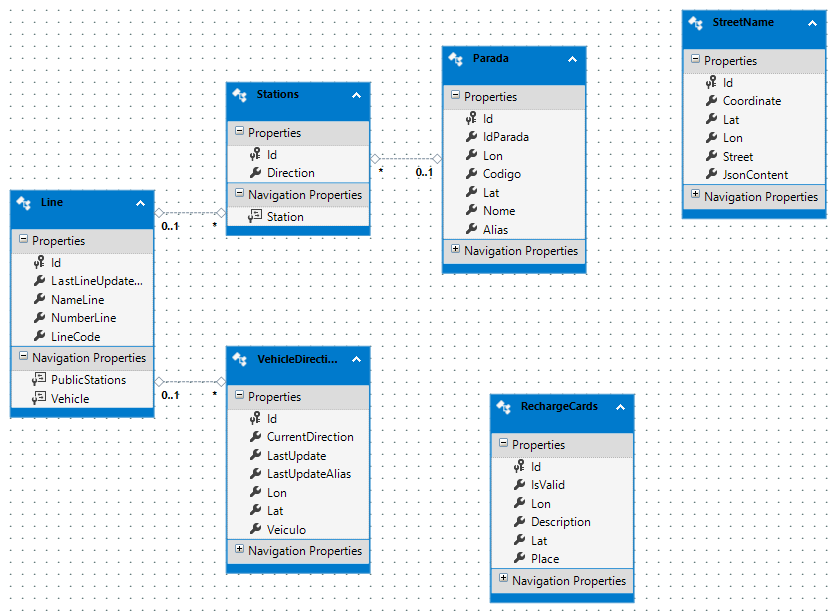
\includegraphics[width=.99\textwidth]{./Resources/EntityDesignerDiagram.png}
\caption{Modelo Visual das classes mapeadas para Objeto-Relacional Section~\ref{sec:Arquitetura}.}
\label{fig:FiguraEsquemaDatabase}
\end{figure}

A figura ~\ref{fig:FiguraEsquemaDatabase} demonstra o esquema do banco de dados utilizado neste trabalho, uma classe principal denominada de Line contém todas as referencias para os objetos que se tem necessidade de expor. Cada linha possui um conjunto de estações que são representadas pela tabela stations, e um conjunto de veículos representados pela tabela VehicleDirection. 

A tabela RechargeCards e StreeName são de suporte a informações gerais, na primeira tabela podemos encontrar dados referentes ao ponto de recarga como Latitude, Longitude, Nome da Rua e se o ponto de venda continua atuante ou válido para seu propósito. A segunda tabela contém a conversão das coordenadas em endereços legíveis.

%%%%%%%%%%%%%%%%% ---------------- Estudo de caso ---------------- %%%%%%%%%%%%%%%%%%
\section{Estudo de caso}
Dada a arquiteura e suas descrições, vamos nesta seção validar a aproximação do modelo real com o modelo proposto no que tange o tempo de espera de cada usuário. 

\subsection{Protótipo de Aplicativo}
Para gerar os dados mensurados nos tópicos ~\ref{sec:tmpDist} e  ~\ref{sec:imprecisao} foi necessário o desenvolvimento de um aplicativo como ferramenta de teste para o modelo criado. A aplicação foi desenvolvida em .NET Core e tem por finalidade fazer requisições das linhas e salvar o conteúdo adquirido do modelo para gerar dados estatísticos.

Os dados gerados são: Hora de chegada real no ponto, hora da última atualização do sistema, tempo estimado de chegada em um ponto definido, sentido, distância estimada e minutos estimados até a chegada. A Tabela contida no endereço XXX contém o resultado de todos os dados analisados, nos tópicos seguinte esses valores serão apresentadas.

\subsection{Estimativa Tempo-Distancia} \label{sec:tmpDist}
Dada uma posição representada por (x,y) onde \textbf{X} representa a latitude e \textbf{Y} a longitude. tem-se um observador na posição Fixa (x,y) e um veiculo de uma linha N qualquer em uma posição (x',y').

Para calcular o quão preciso é o modelo, um observador em (x,y) tem a função de assistir os carros provenientes da Linha N, que tem suas posições variáveis representada por (x',y'). O observador foi inserido na interseção deste caminho que engloba o tráfego em dois sentidos, do bairro ao centro e do centro ao bairro. Este método tenta simular uma requisição de um usuário do sistema de transporte coletivo ao aguardar determinada linha em uma estação. 

Mensura-se então o tempo entre a passagem real do veículo no ponto (x,y), com a estimativa de tempo dada pelo modelo enriquecido. Matematicamente quando esta diferença de tempo se iguala a zero, pode-se dizer que estamos com o melhor índice de precisão, quanto mais este valor se afasta de zero positivamente ou negativamente, menos preciso o sistema se mostra.

Para gerar os dados estatísticos analisou-se uma linha N que contém seis veículos disponíveis durante o dia e a noite, ao todo cinquenta viagens foram analisadas.

\begin{table}[h!]
  \centering
	\begin{tabular}{|c|c|}
      \hline
      Descrição & Resultado \\ \hline
      Variação Média entre tempo real de chegada e tempo estimado & 112 segundos \\ 
      Desvio Padrão entre tempo real de chegada e tempo estimado & 88 segundos \\
      \hline
	\end{tabular}
  \caption{Relação Tempo-Distancia média e com Desvio Padrão.}
  \label{tab:variacoes}
\end{table}

Ao observar apenas as duas grandeza, distância e tempo, foi inferido uma variação média de 112 segundos entre o tempo real de chegada da linha na estação com o tempo de chegada estimado pelo modelos de dados. Portanto, a estimativa que o modelo faz é sensata observando os aspectos descritos em ~\ref{sec:imprecisao}. O Desvio padrão calculado é de aproximadamente 88 segundos. 

\subsection{Intervalo real de atualização de coordenadas sem enriquecimento} \label{sec:CoorVar}

Vamos analisar qual intervalo de tempo entre atualizações de geoposicionamento de cada veiculo, e descreve-los por dois diferentes prismas: O primeiro se concentra na visão do cliente como usuário do sistema de transporte coletivo, e o segundo discorre sobre o trajeto completo e sob os dados informativos que os carros oferecem.

Considera-se neste trabalho a importância da assertividade de tempo ao usuário final do sistema, portanto, mensura-se a ultima atualização do carro ao chegar na posição Fixa (x,y), a qual simula uma estação de ônibus real. Entende-se que a precisão do ultimo trecho é essencial para fidelizar usuários ao sistema.

\begin{table}[h!]
  \centering
	\begin{tabular}{|c|c|}
      \hline
      Descrição & Resultado \\ \hline
      Variação Média de atualização de cada veiculo & 109 segundos \\ 
      Desvio Padrão de atualização de cada veiculo & 128 segundos \\
      \hline
	\end{tabular}
  \caption{Intervalo entre posicionamento real do veiculo com as informações publicadas.}
  \label{tab:variacoesErroTempo}
\end{table}

Foram analisadas 20 viagens que totalizaram uma diferença de 30 minutos, a média de tempo entre atualizações foram de aproximadamente 109 segundos, com desvio padrão de 128 segundos.

A Tabela~\ref{tab:variacoesErroTempo} faz uma analise levando em consideração apenas uma referencia posicional entre o passageiro e a ultima atualização disponibilizada publicamente. Para incrementar esta analise, mapeamos por aproximadamente 5 horas um conjunto de carros e suas atualizações.

\begin{figure}[ht]
\centering
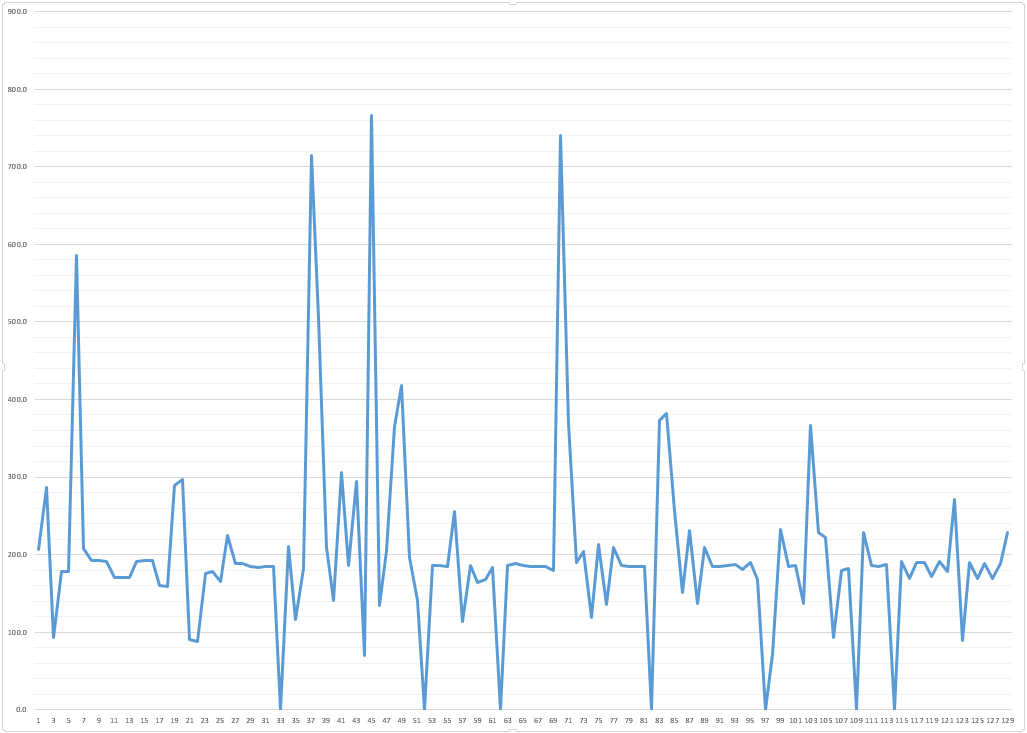
\includegraphics[width=.75\textwidth]{./Resources/GraficoTempo.PNG}
\caption{Gráfico do tempo de atualização. No eixo X a quantidade de atualizações, No eixo Y a variação no tempo medida em segundos. Cada intervalo no eixo Y contém 100 segundos.}
\label{fig:graficoVariacao}
\end{figure}

Os dados coletados informam uma variação média de atualização de 211 segundos. Pode-se afirmar em linhas gerais que cada veiculo irá atualizar sua posição a cada 3.5 minutos. Os dados não seguem um comportamento padrão, a figura~\ref{fig:graficoVariacao} explicita uma acentuada quantidade de dados nos extremos, isto significa que em certos momentos as atualizações são feitas rapidamente, em outros momentos isso demora muito mais do que a média geral.

\subsection{Imprecisão dos dados} \label{sec:imprecisao}
A fonte de dados descrita na seção~\ref{sec:Arquitetura} disponibiliza as informações dos automóveis. Inúmeros são os fatores que podem e alteram a precisão dos dados capturados, serão descritos abaixo os fatores de imprecisão observados durante o experimento.

\begin{enumerate}
\item \textbf{Imprecisão nos dados relatados.} Um automóvel qualquer inerte infere ao seu observador coordenadas distintas em intervalos de tempos distintos. Não houve como inferir a real culpa desta variação porque não foi possível obter acesso ao meio físico, essa alteração não modificou a posição descritiva (nome da rua) do veiculo.\\

\item \textbf{Tempo de resposta entre o carro e o observador.} 
Um automóvel qualquer que parte do ponto X deslocando-se em um tempo T a uma velocidade constante, fornece uma coordenada diferente da coordenada real, visto a variação de espaço, precisão, e tempo de publicação. Pode-se minimizar este comportamento caso a velocidade de troca de informação seja rápida e contínua, o que não foi visto no conjunto estudado. \\

\item \textbf{Velocidade de conexão e exposição dos dados via internet.} A publicação dos dados é feita via internet, normalmente usa-se GPRS para publicar dados de geoposicionamento, porém como não foi possível ter acesso ao meio expositor, O leitor deve atentar-se que esta variação de tempo também deve ser considerada.\\

\item \textbf{Sinistros.} Falhas mecânicas, problemas administrativos ou de segurança podem fazer com que uma linha se torne inoperante, ou que sua rota mude da habitual. Neste tipo de situação as informações se tornam incoerente e falsas, resultando em falsos positivos para os usuários dos dados.\\
\end{enumerate}

%%%%%%%%%%%%%%%%% ---------------- Discussão dos Resultados ---------------- %%%%%%%%%%%%%%%%%%
\section{Discussão dos Resultados}
Neste artigo aplicamos técnicas provenientes de data warehouse com o intuito de enriquecer e agregar valor as informações de transporte coletivo da cidade de manaus. Ao expor as técnicas utilizada e o modelo de dados deu-se um passo a mais para construção de uma cidade inteligente baseada em IOT.

Este trabalho expôs a sociedade uma API com um conjunto de informações sobre o transporte coletivo de manaus, as linhas de ônibus foram mapeadas, suas rotas foram atualizadas e enriquecidas, os pontos de compra de bilhetes de acesso ao modal foram dispostos com informações extras, os carros são monitorados e o modelo descrito tenta aproximar-se ao máximo da realidade para inferir dados mais precisos. Mostrou-se as dificuldades de manter o sistema com alto nível de precisão e as relações que afetam a vida do usuário final do sistema em unidades de tempo e distancia. 

Ao avaliar os tópicos ~\ref{sec:tmpDist} e ~\ref{sec:CoorVar} demonstra-se que as médias de atualização sem o modelo enriquecido é de 211 segundos contra 112 segundos do modelo proposto. Houve um melhoria significativa no tempo de aproximação do modelo real, o que gira em torno de 50\%. No ultimo trecho mapeado entre o veiculo e o usuário do sistema a variação média de atualização foi 109 segundos, e a variação do valor estimado pelo modelo proposto resultou em 112 segundos, portanto, foram extremamente próximos. Pode-se afirmar que na região estudada a informação demonstrada ao usuário tem variação na casa dos dois minutos. 

Dois minutos é um tempo aceitável tendo em vista que o tempo de atualização geral dos veículos é de 3.5 minutos, deve-se ainda observar que o ponto Fixo descrito em~\ref{sec:tmpDist} sofre dos males descritos em~\ref{sec:imprecisao}, mesmo que as variações faça o tempo de atualização aumentar no ultimo trecho, o modelo tem como função corrigir essa variação e continuar informando o usuário com um variação média de 112 segundos.

Ao observar a base de artigos e a base de dados do transporte coletivo da cidade de manaus é possível notar uma defasagem temporal, ou os dados não condizem com a realidade ou são de mais de cinco anos da data deste artigo. Foram integrados dados quantitativos, e reforçou-se os dados qualitativos observados em outras pesquisas como ~\cite{art10} e ~\cite{art11}, portanto a partir deste podemos ver o reflexo da entidade de transporte no ano desta publicação, sanando em partes a defasagem encontrada.

Este trabalho não se encerra em si, esperamos para trabalhos futuros a criação de aplicativos baseados em multiplataformas, como Android, IOS, Windows Universal e para WEB para a exposição de dados. Espera-se simular a pesquisas descritas por ~\cite{art10} com uma quantidade superior de pessoas e retratar de forma mais ampla as características da cidade e da evolução do transporte coletivo.


\bibliographystyle{sbc}
\bibliography{sbc-template}

\end{document}
